%---------------------------------------------------------------------
\section{Separation of Signal from Background Using Matrix Elements}
\label{separation-ME}

\subsection{Method Overview}
\label{method-overview}

The search for single top quark production critically depends on being
able to discriminate between signal-like and background-like events
or, in other words, to perform the optimal test of hypothesis $H_0$:
signal (S), against hypothesis $H_1$: background (B). In this case,
given an event characterized by a set of variables $\vec{x}$, the most
powerful test of hypothesis is given by the Neyman-Pearson test, which
involves a cut on the ratio:
\begin{equation}
\label{disc}
\ell(\vec{x},H_0,H_1) = \frac{P(\vec{x}|H_0)}{P(\vec{x}|H_1)}
= \frac{P_S(\vec{x})}{P_B(\vec{x})},
\end{equation}
\noindent where $P_S(\vec{x})$ and $P_B(\vec{x})$ stand,
respectively, for the signal and background probability density
functions of $\vec{x}$. The power of such a test is also maximal if
the set of variables $\vec{x}$ is complete, in the sense that they
contain all information that is relevant to discriminate between
signal and background. Such optimal test of hypothesis can also be
performed on the a-posteriori Bayesian probability (or Bayes
posterior) of ``$S$ given $\vec{x}$~'' defined as:
\begin{equation}
\label{post}
P(S|\vec{x}) = \frac{P_S(\vec{x})}{P_S(\vec{x}) + P_B(\vec{x})} =
\frac{\ell(\vec{x},S,B)}{\ell(\vec{x},S,B)+1},
\end{equation}
\noindent as it can trivially be expressed in terms of
$\ell(\vec{x},S,B)$.

Many classifiers used in high energy physics, e.g., neural networks,
attempt to approximate $P(S|\vec{x})$, achieving in many cases very
competitive performance. In such methods, significant effort is
devoted at the beginning to selecting the optimal set of variables
that have good discriminating power between signal and
background. This is a time-consuming task, resulting in many instances
in a (not necessarily complete) set of very sophisticated kinematic
and/or topological variables, for which the neural network must try to
learn all correlations in the multi-dimensional space.

The matrix-element-based single top quark search attempts to make use
of all the available kinematic information in the event. Therefore,
$\vec{x}$ represents the set of reconstructed four-momenta for all
selected final state objects in the event. For instance, in the case
of $\ell+$2jets events,
$\vec{x}=(\vec{p}_\ell,\vec{p}_{j1},\vec{p}_{j2})$. The reconstructed
{\met} is not explicitly used, as it results from imposing momentum
conservation in the transverse plane, and thus it does not represent
an independent observable. The method is general enough that
information related to fragmentation or $b$ tagging, can in principle
also be incorporated. In fact, information about the latter is already
being used in the current analysis. In order to achieve optimal
signal-to-background discrimination, given $\vec{x}$, an event
discriminant is defined as:
\begin{equation}
\label{disc2}
D_S(\vec{x}) = P(S|\vec{x})
= \frac{P_S(\vec{x})}{P_S(\vec{x}) + P_B(\vec{x})} 
\end{equation}
\noindent where the signal hypothesis $S$ can be: s-channel $tb$,
t-channel $tqb$, or inclusive $tb$+$tqb$ single top quark
production. The signal and background probability density functions as
a function of $\vec{x}$ are computed numerically based on the
normalized differential cross section for signal and background
processes, respectively. Since the differential cross section for the
process of interest is proportional to the matrix element squared, we
call this method the ``Matrix Element (ME) Method.'' We shall refer to
Eq.~\ref{disc2} as the ``ME discriminant.''

The ME discriminants are evaluated for data events, as well as Monte
Carlo events for the different signal and background
processes. Templates for the ME discriminant distributions
corresponding to the background model are formed and compared to the
same distribution in data, and a binned likelihood as a function of
the signal cross section(s) is computed. A Bayesian method is then
applied to compute the Bayes posterior for the ``signal cross
section(s) given the data'' which, in case of an excess over the
background expectation, can be used to estimate the single top
production cross section(s).
%The significance of the excess is estimated via a measure (p-value)
%of consistency of the observation with the null (background-only)
%hypothesis.


\subsection{Calculation of the Event Probability Density Functions}

The ME event probability density function is defined as the properly
normalized differential cross section for an event characterized by
the reconstructed four-momenta $\vec{x}$:
\begin{equation}
\label{px}
P(\vec{x}) = \frac{1}{\sigma} \times \pderiv{\sigma}{\vec{x}}.
\end{equation}
\noindent These quantities are explained in the following three
sections.

\subsubsection{Differential Cross Section}

The differential cross section, $d\sigma(\vec{x})$ is given in
Eq.~\ref{dsigma}; it is defined as the phase space integration of the
differential cross section at the parton level, convoluted with a
transfer function relating the reconstructed objects to the original
partons.
\begin{equation}
\label{dsigma}
d\sigma(\vec{x}) = \sum_{i,j} \int d\vec{y}
\left[ f_{i}(q_{1}, Q^{2})dq_{1}
\times f_{j}(q_{2}, Q^{2})dq_{2}
\times \pderiv{\sigma_{hs,ij}(\vec{y})}{\vec{y}}
\times W(\vec{x},\vec{y})
\times \Theta_{\rm{Parton}}(\vec{y}) \right]
\end{equation}
\noindent where
\begin{itemize}

\item $\sum_{i,j}$ is a sum of initial parton flavors in the hard
scatter collision. For example, an $s$-channel collision can occur via
$u\bar{d}$, $c\bar{s}$, $d\bar{u}$, or $s\bar{c}$ annihilation.

\item $f_{i}(q, Q^{2})$ is the parton distribution function for parton
$i$ carrying momentum $q$,
evaluated at the factorization scale $Q^2$. For $W$+jets processes we
use $Q^2=M_{W}^{2} + \sum_{jets}({M_{i}^2 + P_{i,T}^2})$ whereas for
single top processes we use $Q^2=m_t^2$. This analysis uses
CTEQ6~\cite{Pumplin:2005rh} leading-order parton distribution
functions via LHAPDF~\cite{LHAPDF}

\item $\partial\sigma_{hs,ij}(\vec{y})/\partial\vec{y}$ is the
differential cross section for the hard scatter collision. This
quantity is proportional to the square of the leading order matrix
element~\cite{PDG} as given by:
\begin{equation}
\label{dsigma_hs}
d\sigma_{hs}
= \frac{(2\pi)^4}{4\sqrt{(q_{1}q_{2})^2 - m_{1}^2m_{2}^2}}
|{\cal M}|^{2}
d\Phi_{n}(\vec{y})
\end{equation}
\noindent where the first term is the flux factor, the second term is
the matrix element squared, and the third term is the $n$-body phase
space factor, with $n=4(5)$ for two-jet (three-jet) events. Matrix
elements in this analysis were obtained from the
Madgraph~\cite{Maltoni:2002qb} leading-order matrix-element generator.

\item $W(\vec{x},\vec{y})$ is called the transfer function, which 
represents the conditional probability of the observed state in the
detector ($\vec{x}$) given the original partons ($\vec{y}$). The
transfer functions are determined using Monte Carlo where the
final-state flavor and four-vector is known. A transfer function is
determined for each jet flavor and for several regions of the
calorimeter. The functions used in this analysis are the same ones
derived and being used in the top mass analysis~\cite{JetTF}. An
example plot of the distribution of the difference between the jet
energy and its parent parton energy, for three types of jets (light,
soft-muon-vetoed $b$-jet and soft-muon-tagged $b$~jet), is shown in
Fig.~\ref{FlavorTF}.

\begin{figure}[!h!tbp]
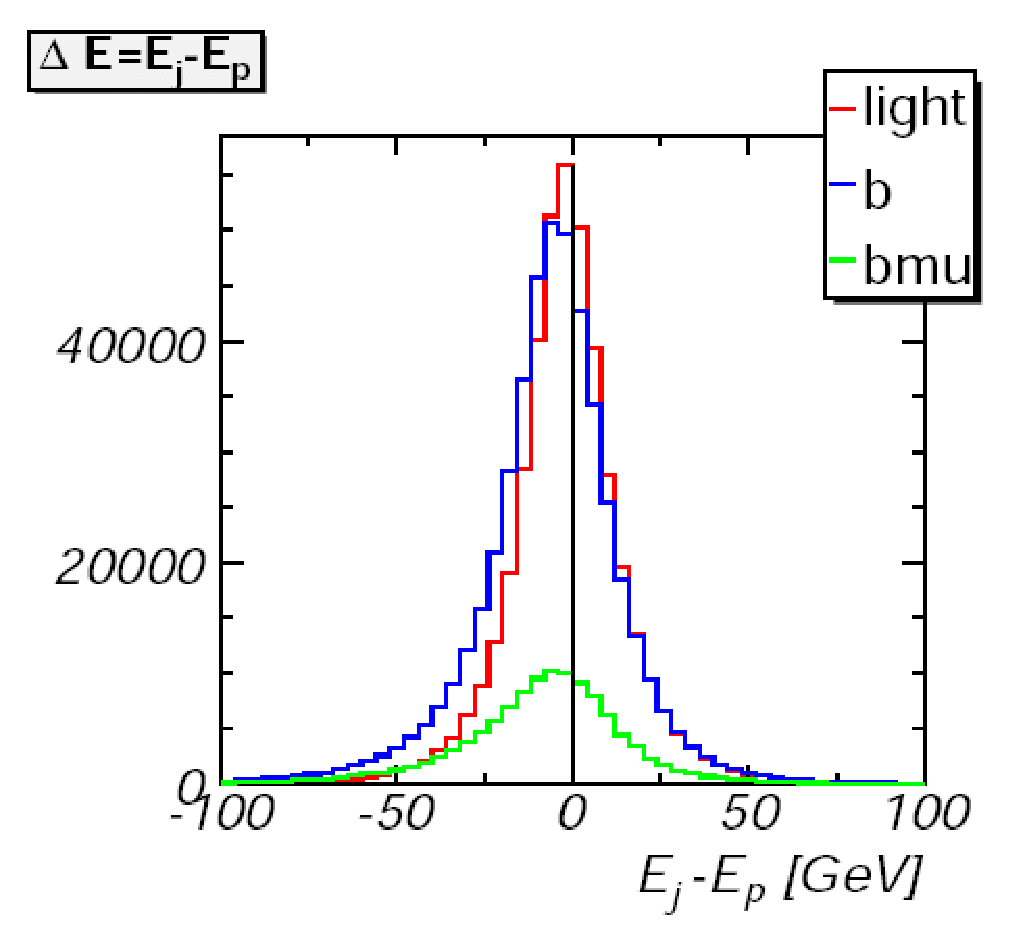
\includegraphics[width=0.4\textwidth]{figures/transfer/tfs}
\vspace{-0.1in}
\begin{minipage}{4in}
\caption[TF]{Energy difference between a jet and its matched parton
for three types of jets for all eta regions and all jet energies.}
\label{FlavorTF}
\end{minipage}
\end{figure}

The electron transfer function is described as a Gaussian distribution
with sigma dependent on the electron energy and
pseudorapidity~\cite{ElectronTF}. The muon transfer functions were
determined for muons with and without an SMT hit and are parametrized
as a function of $1/p_{T}$. The functions used in this analysis are
again the same as the ones used in the top mass
analysis~\cite{MuonTF,MuonTF2}.

\item $\Theta_{\rm{Parton}}(\vec{y})$ represents the parton level
cuts applied in order to avoid singularities in the matrix element
evaluation. These cuts are looser than the corresponding cuts at the
reconstructed level. All cross sections were calculated with the
following parton level cuts:

\begin{itemize}
\item Parton isolation: $\Delta$R($q_{i}$,$q_{j})>0.5$
\item Minimum parton $P_T$: $P_{T}(q_i)>6$ GeV
\item Maximum parton pseudorapidity: $|\eta(q_i)|<3.5$
\item No cuts applied to the lepton or neutrino
\end{itemize}

\item $\int d\vec{y}dq_{1}dq_{2}$ is an integration over the matrix
element phase space. The matrix element phase space for two parton
final state events is defined by the 14 independent spatial degrees of
freedom for the lepton, neutrino, and two partons as shown in
Eq.~\ref{dy}
\begin{equation}
\label{dy}
d\vec{y}_{2} = dq_{1}dq_{2}d|p|_{\ell}
d\Omega_{\ell}d|p|_{\nu}
d\Omega_{\nu}d|p|_{q1}
d\Omega_{q1}d|p|_{q2}
d\Omega_{q2}
\end{equation}

Events with three partons in the final state have 17 independent
degrees of freedom and has a phase space defined in Eq.~\ref{dy3jet}.
\begin{equation}
\label{dy3jet}
d\vec{y}_{3} = dq_{1}dq_{2}d|p|_{\ell}
d\Omega_{\ell}d|p|_{\nu}
d\Omega_{\nu}d|p|_{q1}
d\Omega_{q1}d|p|_{q2}
d\Omega_{q2}d|p|_{q3}
d\Omega_{q3}
\end{equation}

Four (six) degrees of freedom are removed from the integration for two
(three) parton event by assuming equal angles for partons and
jets. This approximation has been verified in Monte Carlo. Two more
degrees of freedom are removed by assuming well measured lepton
angles. Four more degrees of freedom are removed from the integration
by energy-momentum conservation, leaving four integration
variables. The final integration phase space is then transformed to
suit the matrix element being integrated. $W$+jets matrix element
integrations use the phase space defined in Eqs.~\ref{wjets_int} and
single top matrix element integrations use the phase space in
Eq.~\ref{st_int}. The phase space for events with three jets is shown
in Eq.~\ref{wjets_int_3jet} and~\ref{st_int_3jet}.
\begin{equation}
\label{wjets_int}
d\vec{y}_{\rm{W+jets - 2jets}}
= dr_{W}d|p_{q1}|d|p_{q2}|dp^{system}_{z}
\end{equation}
\begin{equation}
\label{st_int}
d\vec{y}_{\rm{single top - 2jets}} = dr_{\rm{top}}
dr_{W}d|p_{q2}|dp^{system}_{z}
\end{equation}
\begin{equation}
\label{wjets_int_3jet}
d\vec{y}_{\rm{W+jets - 3jets}}
= dr_{W}d|p_{q1}|d|p_{q2}|d|p_{q3}|dp^{system}_{z}
\end{equation}
\begin{equation}
\label{st_int_3jet}
d\vec{y}_{\rm{single top - 3jets}}
= dr_{\rm{top}}dr_{W}d|p_{q2}|d|p_{q3}|dp^{system}_{z}
\end{equation}
\noindent 
where $dr_{W}$ and $dr_{\rm{top}}$ are used to uniformly sample a Breit-Wigner distribution from the square of the
invariant mass distribution for $W$~boson and top quark production,
respectively. This choice of sampling minimizes integration time because the
matrix elements for these processes are negligable in regions where the invariant
mass of the lepton and neutrino is far from the $W$ mass and similarly for top
events where the mass of the lepton, neutrino, and $b$-quark is far from the top
mass. More information regarding the choice of variables and
the multidimensional integration can be found in
Appendix~\ref{full}. The multidimensional integrals were calculated
using the GNU~\cite{GNU} Scientific Library's version of the VEGAS
Monte Carlo integration technique~\cite{Lepage:1980dq}.

\end{itemize}

\subsubsection{Matrix Element Processes}

For events with exactly two jets, we consider a total of five matrix
elements for $2{\rar}4$ processes (top quark and $W$ bosons are
treated off-shell): s-channel single top ($ud{\rar}tb$), t-channel
single top ($ub{\rar}td$), $Wbb$ production ($ud{\rar}Wb\bar{b}$),
$Wcg$ production ($sg{\rar}Wcg$), and $Wgg$ production
($ud{\rar}Wgg$). ``tqb'' is used sometimes when referring to t-channel
events because the main diagram that describes these events is the
2$\rar$5 diagram with ``tqb'' in the final state. This analysis uses a
2$\rar$4 diagram with ``tq'' as the final state, as seen in
Fig~\ref{2jets}, because events with two jets require at most two
quarks or gluons in the final state. The three $W$+jets matrix
elements were chosen by running the Madgraph Monte Carlo generator and
selecting those processes which gave the largest cross section after
an overall $b$-tagging efficiency was applied. The leading order
diagrams for these channels (displayed as $2{\rar}3$ processes for
simplicity) are shown in Fig.~\ref{2jets}.

For events with three jets, we consider a total of three matrix
elements: s-channel single top ($ud{\rar}tbg$), t-channel single top
($ug{\rar}tbd$), and $Wbb$ production ($ud{\rar}Wb\bar{b}g$). The
number of $W$+jets matrix elements considered has been limited due to
the significant time required to compute the differential cross
section in Eq.~\ref{dsigma}. As will be discussed in
Section~\ref{disc-def}, this can only result in a reduced sensitivity
but does not affect the validity of the analysis. The leading order
diagrams for these channels (displayed as $2{\rar}3,4$ processes for
simplicity) are shown in Fig.~\ref{3jets}.

\clearpage

\begin{figure}[!h!tbp]
\includegraphics[width=0.27\textwidth]{figures/feynman/tb}
\hspace{0.2in}
\includegraphics[width=0.27\textwidth]{figures/feynman/tq}\\
\includegraphics[width=0.27\textwidth]{figures/feynman/wbb}
\hspace{0.2in}
\includegraphics[width=0.27\textwidth]{figures/feynman/wcg}
\hspace{0.2in}
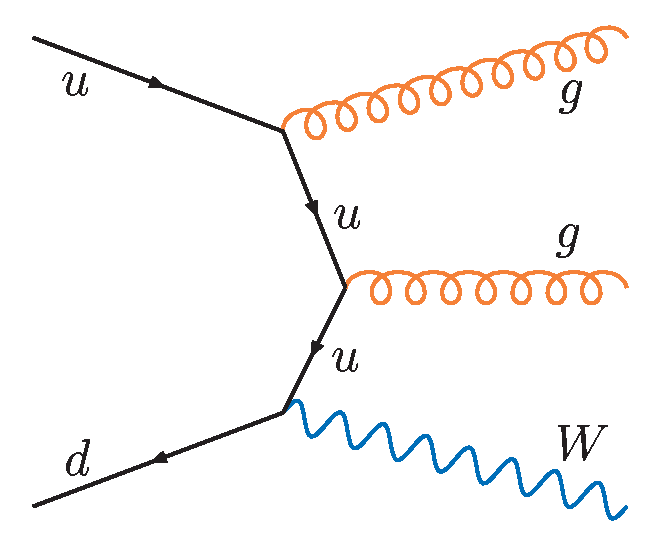
\includegraphics[width=0.27\textwidth]{figures/feynman/wgg}
\caption[2jets]{Representative Feynman diagrams corresponding to 
the leading-order matrix elements used for event probability
calculation for events with exactly two jets. Upper row, signals:
$ud{\rar}tb$, $ub{\rar}td$; lower row, backgrounds: $ud{\rar}Wbb$,
$sg{\rar}Wcg$, $ud{\rar}Wgg$.}
\label{2jets}
\end{figure}

\begin{figure}[!h!tbp]
\includegraphics[width=0.24\textwidth]{figures/feynman/tbg}
\hspace{0.2in}
\includegraphics[width=0.24\textwidth]{figures/feynman/tqb}
\hspace{0.2in}
\includegraphics[width=0.24\textwidth]{figures/feynman/wbbg}
\caption[3jets]{Representative Feynman diagrams corresponding to 
the leading-order matrix elements used for event probability
calculation for events with exactly three jets. Left two plots:
signals, $ud{\rar}tbg$, $ug{\rar}tbd$; right plot:
background,$ud{\rar}Wbbg$.}
\label{3jets}
\end{figure}

\subsubsection{Cross Section}

The event probability density function defined in Eq.~\ref{px}
requires a normalization constant to retain the probability density
interpretation. The normalization constant $\sigma$ is defined as the
detector level phase space integration $\int d\vec{x}$ of the
differential cross section defined in Eq.~\ref{dsigma}.
\begin{equation}
\label{cross}
\sigma = \sum_{i,j} \int d\vec{x}d\vec{y}
\left[ \pderiv{\sigma_{i,j}(\vec{y})}{\vec{y}}
\times W(\vec{x},\vec{y})
\times \Theta_{\rm{cuts}}(\vec{x})
\right]
\end{equation}
\noindent Because all the events for which the probability density
will be computed have had selection cuts applied, it is necessary to
consider this in the calculation of the cross section. The term
$\Theta_{\rm{cuts}}(\vec{x})$ is included in the calculation to
simulate the selection cuts. All cross sections were calculated with
the following selection cuts:

\begin{myitemize}
\item Lepton $P_{T}$ $>$ 15 GeV
\item Electron (muon) $|\eta|$ $<$ 1.1(2.0)
\item Missing $E_{T}$ $>$ 15 GeV
\item Leading jet $P_{T}$ $>$ 25 GeV
\item Leading jet $|\eta|$ $<$ 2.5
\item Second jet $P_{T}$ $>$ 20 GeV
\item Second jet $|\eta|$ $<$ 3.5
\item Third jet $P_{T}$ $>$ 20 GeV (if three-jet event)
\item Third jet $|\eta|$ $<$ 3.5 (if three-jet event)
\end{myitemize}

The selection cuts shown above are slighty different from the
canonical single top cuts. These cuts are included in the
normalization calculation to approximate the relative acceptance
difference between signal and background events. The cross sections
computed for each signal and background process for two- and three-jet
events are summarized in Table~\ref{cross-sections}. In all instances,
the statistical uncertainty from the Monte Carlo integration is below
$1\%$.

\begin{table}[!h!tbp]
\begin{center}
\begin{minipage}{5.5 in}
\begin{ruledtabular}
\begin{tabular}{l||cccccccc}
\multicolumn{9}{c}
{\underline{Cross Section $\times$ Branching Fraction [fb]}}
\vspace{0.05in} \\
            & \multicolumn{4}{c}{2-jet events}
            & \multicolumn{4}{c}{3-jet events} \\
            & \multicolumn{2}{c}{1 tag}
            & \multicolumn{2}{c}{2 tags}
            & \multicolumn{2}{c}{1 tag}
            & \multicolumn{2}{c}{2 tags}\\
            & Electron &   Muon   & Electron &   Muon
            & Electron &   Muon   & Electron &   Muon   \\
\hline
Signals     &    &     &     &    &    &     &    &     \\
~~$tb(g)$   &   8.07   &   10.4   &   6.90   &   8.90   
            &   6.02   &   7.64   &   5.22   &   6.66   \\
~~$tq(b)$   &  19.6    &   26.8   &   0.27   &   0.38   
            &   6.34   &    8.56  &   5.40   &   7.40   \\
Backgrounds &    &     &     &    &    &     &    &     \\
~~$Wbb(g)$  &  29.5    &   41.9   &  24.6    &  34.7    
            &   6.34   &   8.56   &   5.40   &   7.40   \\
~~$Wcg$     &  36.4    &   54.0   &   0.33   &   0.61   & & & & \\
~~$Wgg$     &  52.3    &   74.5   &   0.33   &   0.47   & & & &  
\end{tabular}
\end{ruledtabular}
\vspace{-0.1 in}
\caption[xsecs]{Cross section times branching fraction for each
analysis channel.}
\label{cross-sections}
\end{minipage}
\end{center}
\end{table}


\subsubsection{Treatment of Combinatorial Background}

The event probability density shown in Eq.~\ref{px} assumes a known
assignment between a jet and parton from the matrix element. In
practice, this assignment is not a-priori known and we must sum over
all possible assignments. In general, the event differential cross
section is modified as shown in Eq.~\ref{pxcomb}:
\begin{eqnarray}
\label{pxcomb}
d\sigma(\ell, j_1, j_2)
&=& \alpha_{j_1 {\rar} p_1} \alpha_{j_2 {\rar} p_2}
    d\sigma(\ell, j_1 {\rar} p_1, j_2 {\rar} p_2) + \nonumber \\
&+& \alpha_{j_2 {\rar} p_1} \alpha_{j_1 {\rar} p_2}
    d\sigma(\ell, j_2 {\rar} p_1, j_1 {\rar} p_2) 
\end{eqnarray}
\noindent where the $\alpha$ parameters relate to the probability of
the jet-parton match. If there is no a-priori knowledge of the correct
assignment, these quantities can be made equal. Thereby no preference
is given to either assignment.

This analysis uses information from the neural network
$b$~tagger~\cite{NNbtag} to weight the different jet-parton
combinations depending on whether a given jet is tagged or not and
which parton flavor is being assigned to it when summing over the
combinatorial background (see Eq.~\ref{pxcomb}). Therefore the
$\alpha$ weights are related to the jet tag-rate functions for the
different hypothesized jet flavors ($b$, $c$ and light), as shown in
Table~\ref{jp}. The different jet tag-rate functions for each flavor
have been provided by the B-ID group parametrized in terms of jet
$P_T$ and $\eta$: $\varepsilon_{\rm flavor}(j)=\varepsilon_{\rm
flavor}(P_T(j),\eta(j))$.

\begin{table}[!h!tbp]
\begin{center}
\begin{minipage}{3 in}
\begin{ruledtabular}
\begin{tabular}{c||cc}
\multicolumn{3}{c}
{\underline{Jet-Parton Matching Weight Factors}}\vspace{0.05in} \\
Parton flavor  &     $b$ tagged    &      Not tagged       \\
\hline
$b$            & $\varepsilon_{b}$ &  $1-\varepsilon_{b}$  \\
$c$            & $\varepsilon_{c}$ &  $1-\varepsilon_{c}$  \\
light          & $\varepsilon_{l}$ &  $1-\varepsilon_{l}$
\end{tabular}
\end{ruledtabular}
\vspace{-0.1 in}
\caption[jp]{Weights for the event differential cross section
depending on the $b$-tagging status of the jet and jet-parton
assignment.}
\label{jp}
\end{minipage}
\end{center}
\end{table}

For example, let us assume we have a given two-jet event with $j_1$
tagged and $j_2$ not tagged, and we are trying to evaluate the
probability density function for the $Wcg$ hypothesis, summing over
the two possible jet-parton assignments. In this case, the
differential cross section would be given by:
\begin{eqnarray}
\label{pxcomb_wcg}
d\sigma_{Wcg}(\ell, j_1, j_2)
&=& \varepsilon_{c}(j_1)(1-\varepsilon_{l}(j_2))
d\sigma_{Wcg}(\ell, j_1 {\rar} c, j_2 {\rar} g) + \nonumber \\ 
&+& \varepsilon_{l}(j_2))(1-\varepsilon_{c}(j_1))
d\sigma_{Wcg}(\ell, j_2 {\rar} c, j_1 {\rar} g).
\end{eqnarray}

This differential cross section must then be integrated over the
reconstructed lepton and jets four-momenta in order to compute the
event probability density function.

\subsection{Single Top Discriminant}

\subsubsection{Discriminant Definition}
\label{disc-def}

As discussed in Section~\ref{method-overview}, the signal and
background probability density functions are used to build an event
discriminant, defined in Eq.~\ref{disc2}. In particular, it is
possible to define discriminants specific to each of the single
top production modes, as well as inclusive for single top production, 
assuming the SM ratio of $s$- and $t$-channel cross sections.

The channel-specific discriminants are defined as:
\begin{equation}
D_{tb(tqb)}(\vec{x})
= \frac{P_{tb(tqb)}(\vec{x})}{P_{tb(tqb)}(\vec{x}) + P_{B}(\vec{x})}.
\label{disc1d}
\end{equation}
\noindent where $tqb$ here generically refers to the $t$-channel
process, whether based on the $tq$ matrix elements (two-jet events) or
the $tqb$ matrix elements (three-jet events).

%
% AJ 11/18/2006
% Comment this out since we won't be showing yet results from the
% tb+tqb discriminant
%
%The inclusive $tb$+$tqb$ discriminant is defined as:
%\begin{equation}
%D_{tb+tqb}(\vec{x})
%= \frac{\rho_{tb}P_{tb}(\vec{x})+(1-\rho_{tb})P_{tqb}(\vec{x})}
%{\rho_{tb}P_{tb}(\vec{x})+(1-\rho_{tb})P_{tqb}(\vec{x}) + P_{B}
%(\vec{x})},
%\label{disc1d_tbtqb}
%\end{equation}
%\noindent where $\rho_{tb}$ represents the expected 
%fraction of signal events from $s$-channel production after
%selection, which is
%computed for the different analysis channels and assuming the SM
%prediction
%of $\sigma_{tb}/\sigma_{tqb}=0.44$ (see Table~\ref{rhotb}).
%
%\vspace{0.05in}
%\begin{table}[!h!tbp]
%\begin{center}
%\begin{minipage}{3 in}
%\begin{ruledtabular}
%\begin{tabular}{l||cccc}
%\multicolumn{5}{c}
%{\hspace{0.5in}\underline{Expected $tb$ Fraction}}
%\vspace{0.1in} \\
%           & \multicolumn{2}{c}{1 tag} & \multicolumn{2}{c}{2 tags}\\
%           & Electron &   Muon   & Electron &   Muon   \\
%\hline
%2jet  &  {\color{red} X.XX}  &{  \color{red} X.XX}  
%5&  {\color{red} X.XX}  &  {\color{red} X.XX}  \\   
%3jet  &  {\color{red} X.XX}  &{  \color{red} X.XX}  
%&  {\color{red} X.XX}  &  {\color{red} X.XX}  \\    
%\end{tabular}
%\end{ruledtabular}
%\vspace{-0.1 in}
%\caption[rhotb]{Expected $tb$ fraction in selected single top
%events.}
%\label{rhotb}
%\end{minipage}
%\end{center}
%\end{table}

For two-jet events, the background probability density function
$P_B(\vec{x})$ is given by:
\begin{equation}
P_{B}(\vec{x})= C_{Wbb}P_{Wbb}(\vec{x})
              + C_{Wcg}P_{Wcg}(\vec{x})
              + C_{Wgg}P_{Wgg}(\vec{x}),
\label{probb}
\end{equation}
\noindent where $C_{Wbb}$, $C_{Wcg}$, and $C_{Wgg}$ are, in
principle, the relative fractions of each background in the
data. However, as discussed below, these background fractions are
optimized for the analysis.

The background fractions for the two-jet discriminant were found by a
grid search of each point ($C_{Wbb}$, $C_{Wcg}$, $C_{Wgg}$) and
calculating the expected Bayes ratio defined as the maximum of the
two-dimensional posterior divided by the value of the posterior at
zero signal cross section. This procedure was used by each analysis in
the single top group to optimize the final discriminant variable. The
values of the background fractions are summarized in Table~\ref{frac}.

\begin{table}[!h!tbp]
\begin{center}
\begin{minipage}{3 in}
\begin{ruledtabular}
\begin{tabular}{l||cccc}
\multicolumn{5}{c}
{\hspace{0.5in}\underline{Optimized Background Fractions}}
\vspace{0.1in} \\
           & \multicolumn{2}{c}{1 tag} & \multicolumn{2}{c}{2 tags}\\
           & Electron &   Muon   & Electron &   Muon   \\
\hline
$C_{Wbb}$  &   0.20   &   0.40   &   0.67   &     1    \\
$C_{Wcg}$  &   0.40   &   0.40   &     0    &     0    \\
$C_{Wgg}$  &   0.40   &   0.20   &   0.33   &     0
\end{tabular}
\end{ruledtabular}
\vspace{-0.1 in}
\caption[frac]{Background fractions chosen for each analysis channel
in two-jet events.}
\label{frac}
\end{minipage}
\end{center}
\end{table}

For the three-jet analysis, the background probability density
function $P_B(\vec{x})$ is given by:
\begin{equation}
P_{B}(\vec{x})= P_{Wbbg}(\vec{x}),
\label{probb_3j}
\end{equation}
\noindent which represents a further step in simplification relative
to the two-jet analysis.

At this point, a remark is in order. As can be seen, the background
probability density function does not contain multijet or $t\bar{t}$
matrix elements. Even for the case of $W$+jets, some simplifications
are made regarding which processes to consider and the relative
contributions of each of them to the total background probability
density. It should be stressed that the result of such approximations
can only be reduced discrimination. The background model still
contains all processes and the event discriminant is computed for all
of them to build the templates that will be compared to data.

\subsubsection{One-Dimensional Discriminants}

This section contains overlayed plots of the one-dimensional (1D) $tb$
and $tq$ discriminants for signal and background events. The events in
the plots come from the combined $e$,$\mu$ / 1,2 tags / 2,3 jets
channel. Figures~\ref{disc_wbb} and \ref{disc_wjets} show good
discrimination between signal and $W$+jets or multijets backgrounds.
However, the discrimination is poorer between signal and $\dilepton$
and $\lepjets$ events as shown in Fig.~\ref{disc_ttbar}. The lack of
discrimination power for $\ttbar$ events is due to the fact that the
current version of the analysis does not yet include a $\ttbar$
probability density function in the definition of the discriminant.
The $\ttbar$ matrix element takes much longer to integrate because
there are six partons in the final state while there are four in the
single top and $W$+jets matrix elements. Adding a $\ttbar$ matrix
element is envisioned as a future improvement for this analysis.

\begin{figure}[!h!tbp]
\includegraphics[width=0.40\textwidth]
{figures/performance/tb_Discriminant__schannel_wbb}
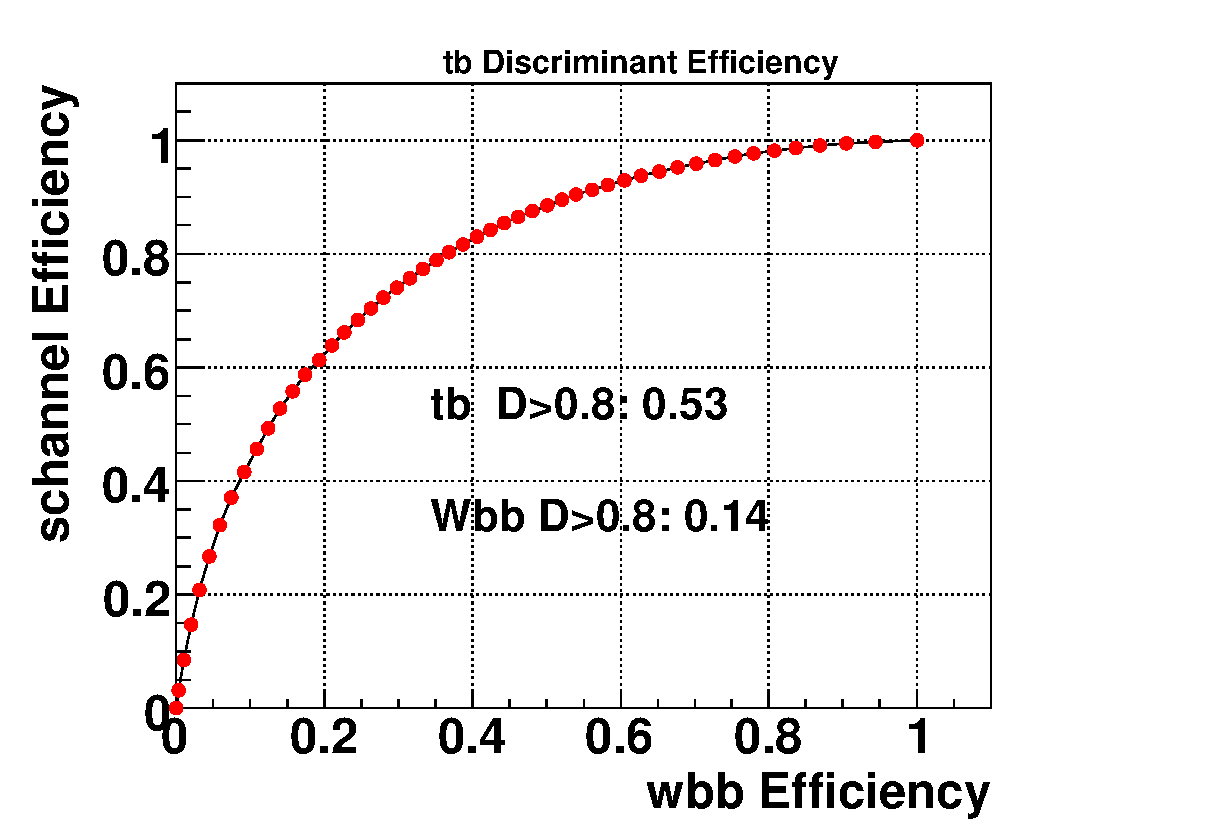
\includegraphics[width=0.40\textwidth]
{figures/performance/tb_Efficiency__schannel_wbb}
\includegraphics[width=0.40\textwidth]
{figures/performance/tb_Discriminant__schannel_wcc}
\includegraphics[width=0.40\textwidth]
{figures/performance/tb_Efficiency__schannel_wcc}
\includegraphics[width=0.40\textwidth]
{figures/performance/tq_Discriminant__tchannel_wbb}
\includegraphics[width=0.40\textwidth]
{figures/performance/tq_Efficiency__tchannel_wbb}
\includegraphics[width=0.40\textwidth]
{figures/performance/tq_Discriminant__tchannel_wcc}
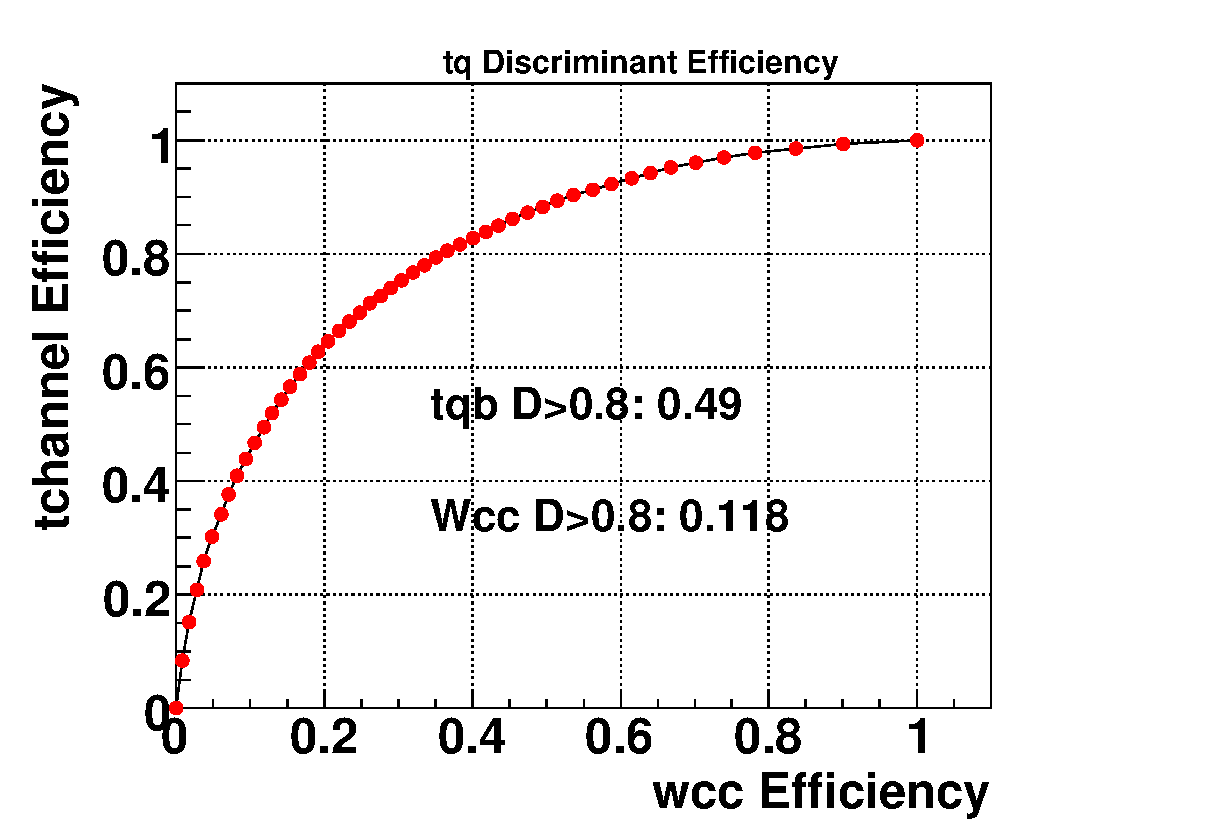
\includegraphics[width=0.40\textwidth]
{figures/performance/tq_Efficiency__tchannel_wcc}
\caption[discwbb]{Discriminant plots and efficiency curves for:
first row, $tb$ vs. $Wbb$, second row, $tb$ vs. $Wcc$, third row, $tq$
vs. $Wbb$, and fourth row, $tq$ vs. $Wcc$. The numbers in the
efficiency curves (right column) represent the fraction of signal or
background the remains after a discriminant cut of 0.8.}
\label{disc_wbb}
\end{figure}

\begin{figure}[!h!tbp]
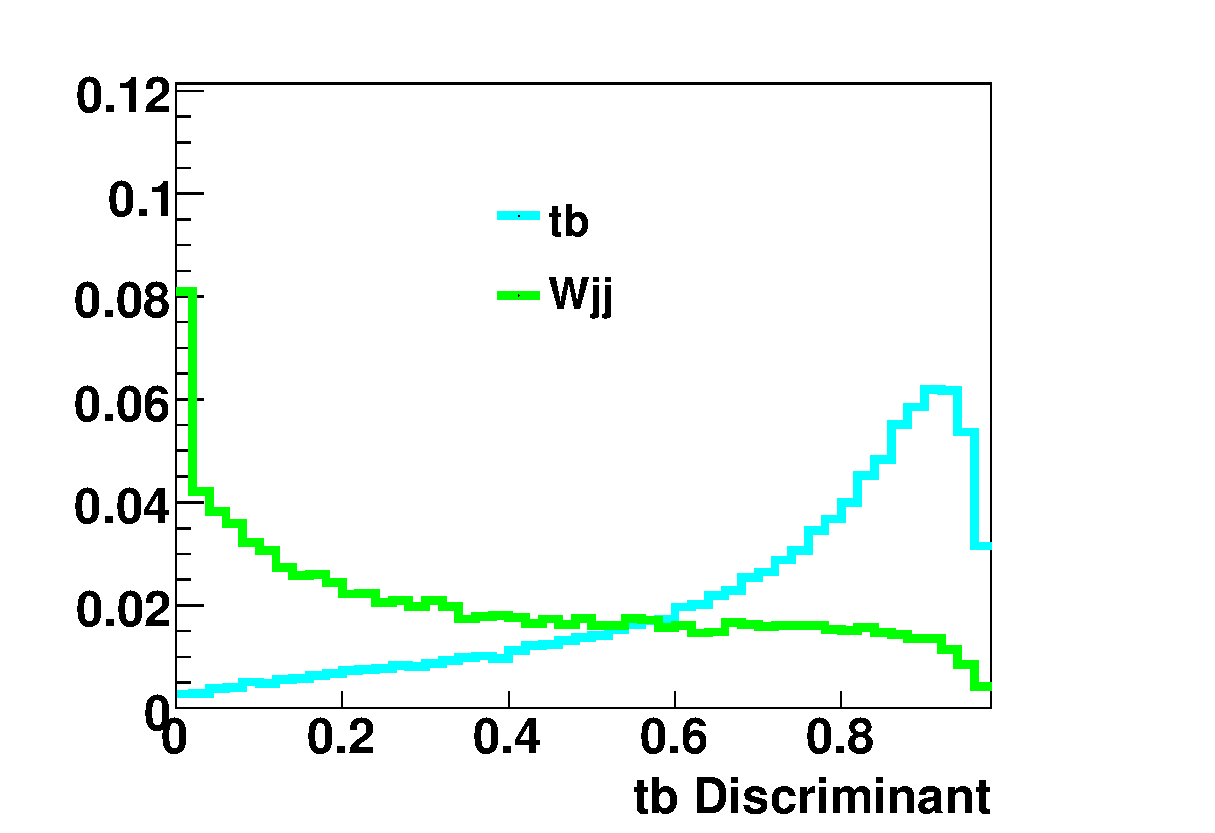
\includegraphics[width=0.40\textwidth]
{figures/performance/tb_Discriminant__schannel_wjj}
\includegraphics[width=0.40\textwidth]
{figures/performance/tb_Efficiency__schannel_wjj}
\includegraphics[width=0.40\textwidth]
{figures/performance/tb_Discriminant__schannel_qcd}
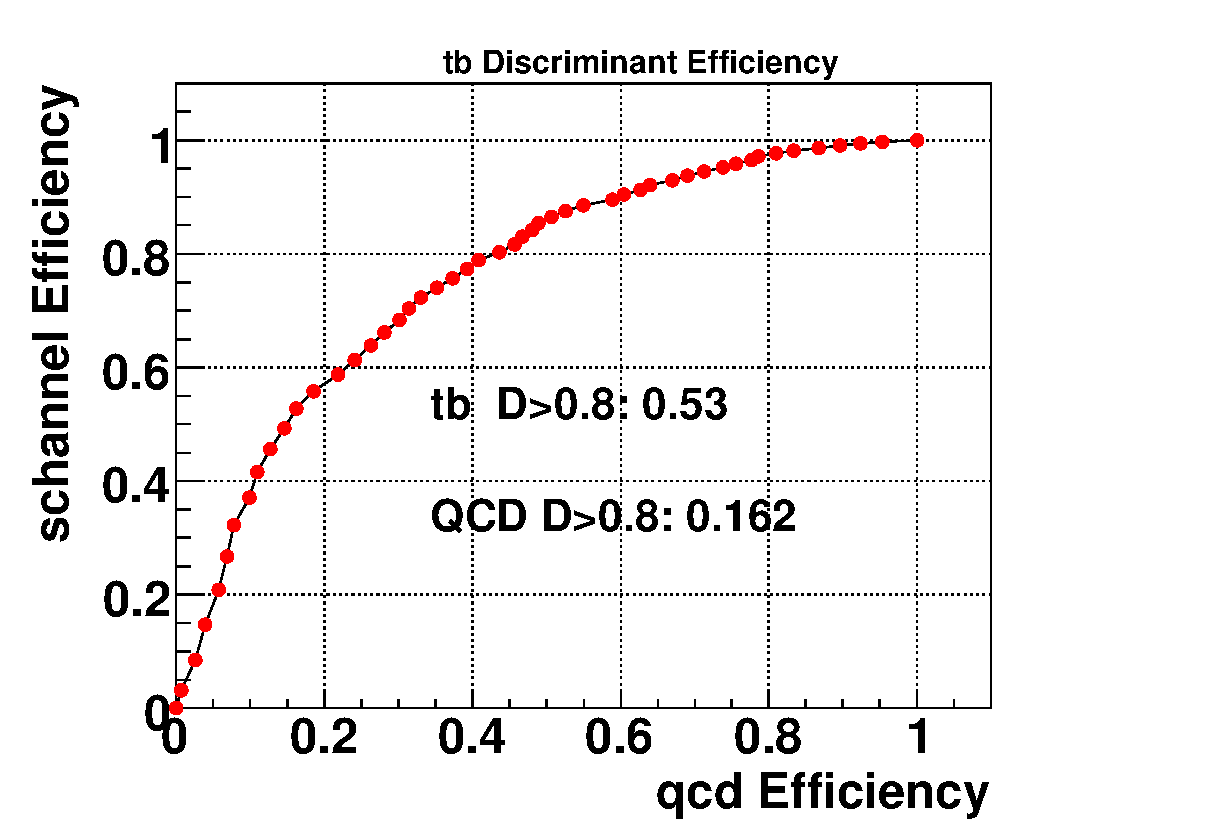
\includegraphics[width=0.40\textwidth]
{figures/performance/tb_Efficiency__schannel_qcd}
\includegraphics[width=0.40\textwidth]
{figures/performance/tq_Discriminant__tchannel_wjj}
\includegraphics[width=0.40\textwidth]
{figures/performance/tq_Efficiency__tchannel_wjj}
\includegraphics[width=0.40\textwidth]
{figures/performance/tq_Discriminant__tchannel_qcd}
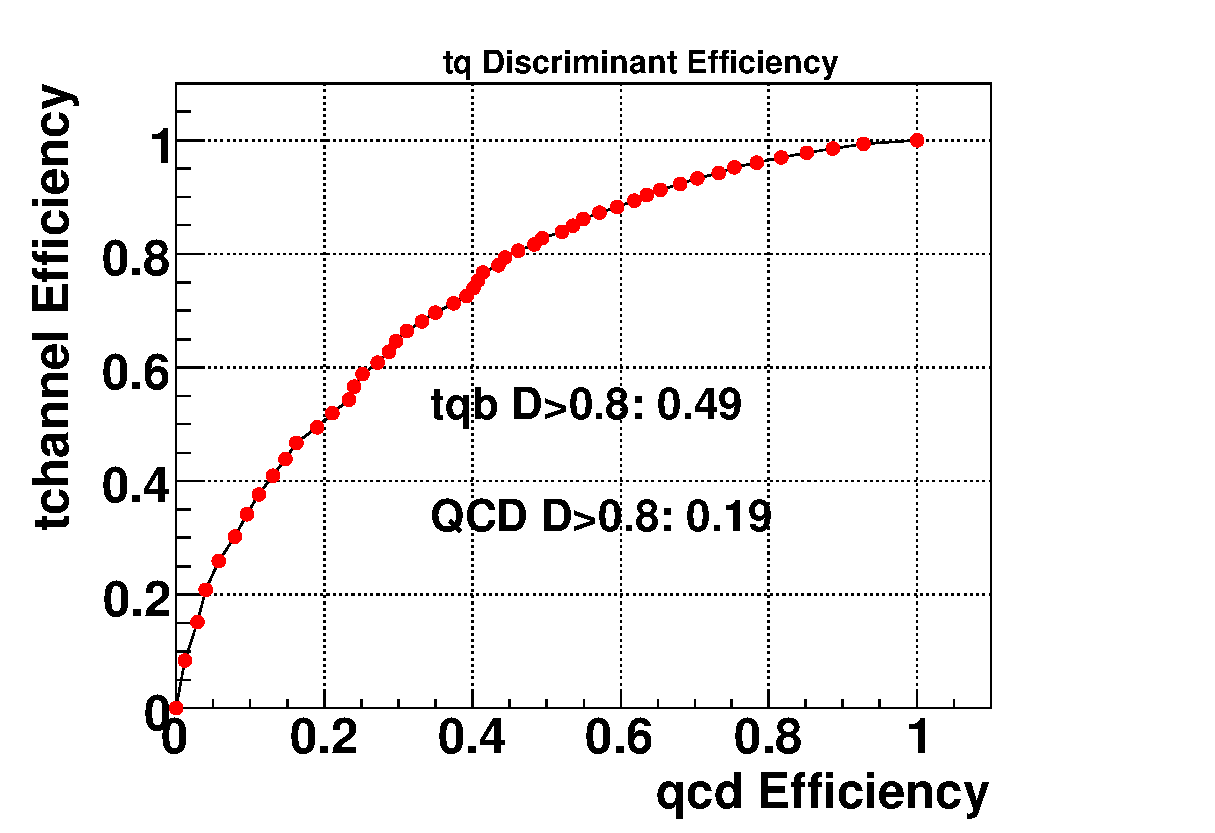
\includegraphics[width=0.40\textwidth]
{figures/performance/tq_Efficiency__tchannel_qcd}
\caption[discwjets]{Discriminant plots and efficiency curves for:
first row, $tb$ vs. $Wjj$, second row, $tb$ vs. multijets, third row,
$tq$ vs. $Wjj$, and fourth row, $tq$ vs. multijets. The numbers in the
efficiency curves (right column) represent the fraction of signal or
background the remains after a discriminant cut of 0.8.}
\label{disc_wjets}
\end{figure}

\begin{figure}[!h!tbp]
\includegraphics[width=0.40\textwidth]
{figures/performance/tb_Discriminant__schannel_dilepton}
\includegraphics[width=0.40\textwidth]
{figures/performance/tb_Efficiency__schannel_dilepton}
\includegraphics[width=0.40\textwidth]
{figures/performance/tb_Discriminant__schannel_lepjets}
\includegraphics[width=0.40\textwidth]
{figures/performance/tb_Efficiency__schannel_lepjets}
\includegraphics[width=0.40\textwidth]
{figures/performance/tq_Discriminant__tchannel_dilepton}
\includegraphics[width=0.40\textwidth]
{figures/performance/tq_Efficiency__tchannel_dilepton}
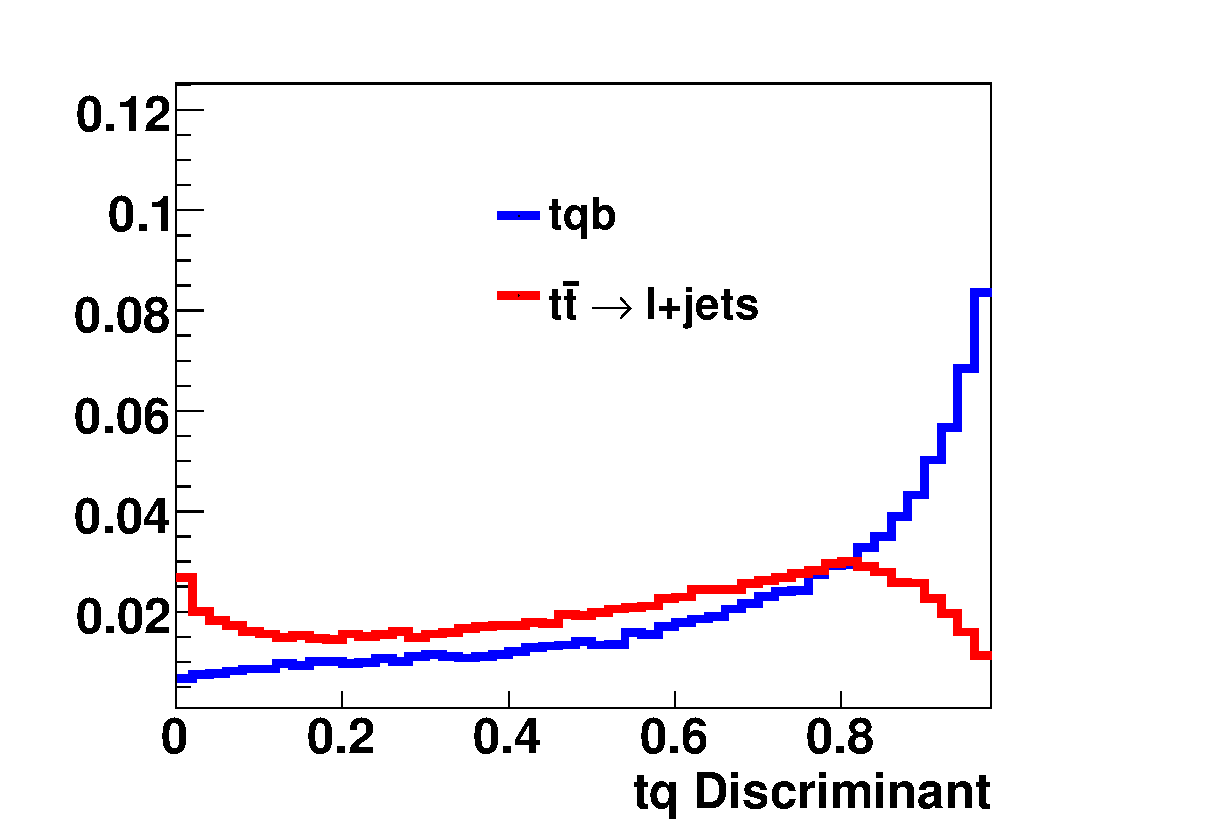
\includegraphics[width=0.40\textwidth]
{figures/performance/tq_Discriminant__tchannel_lepjets}
\includegraphics[width=0.40\textwidth]
{figures/performance/tq_Efficiency__tchannel_lepjets}
\caption[discttbar]{Discriminant plots and efficiency curves for:
first row, $tb$ vs. $\dilepton$, second row, $tb$ vs. $\lepjets$,
third row, $tq$ vs. $\dilepton$, and fourth row, $tq$
vs. $\lepjets$. The numbers in the efficiency curves (right column)
represent the fraction of signal or background the remains after a
discriminant cut of 0.8.}
\label{disc_ttbar}
\end{figure}

\subsubsection{Two-Dimensional Discriminants}

This analysis uses a two-dimensional (2D) discriminant computed from
the 1D $tb$ and $tq$ discriminants discussed in the previous
section. The 2D discriminant is more powerful than either 1D
projection because it selects events with both $tb$ and $tq$
characteristics, which helps to further reduce the $W$+jets and
$\ttbar$ background which may have either characteristic but not
necessarily both. 
%Furthermore, the simultaneous sensitivity to both
%production channels makes the 2D discriminant an essential tool to
%perform a model-independent search and/or cross section measurement,
%without having to make assumptions about e.g., the $tb$:$tq$ cross
%section ratio. 

Figures~\ref{wbbwccwjj} and \ref{qcdtt} show the 2D discriminants
for single top quark signals and for all the backgrounds. The
plots are normalized to unit volume.

\clearpage

\begin{figure}[!h!tbp]
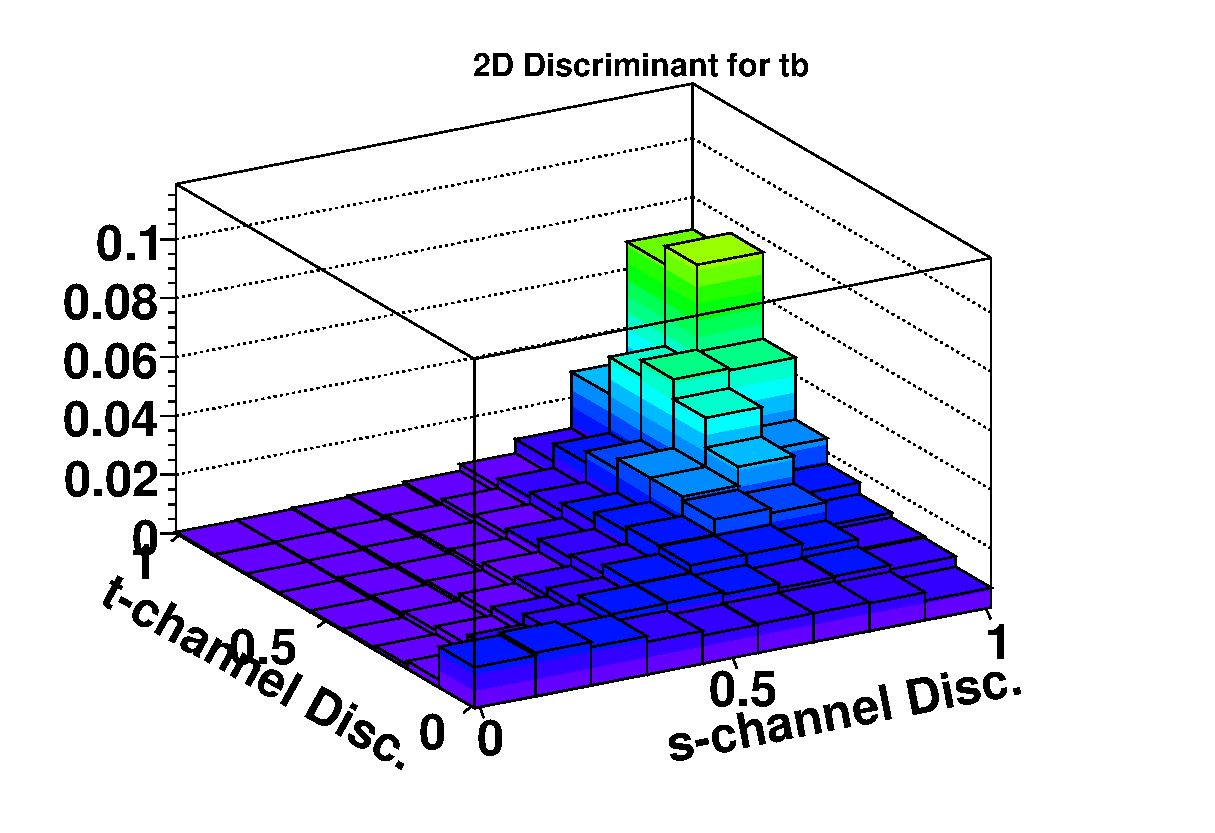
\includegraphics[width=0.32\textwidth]
{figures/performance/2D-Discriminant_schannel}
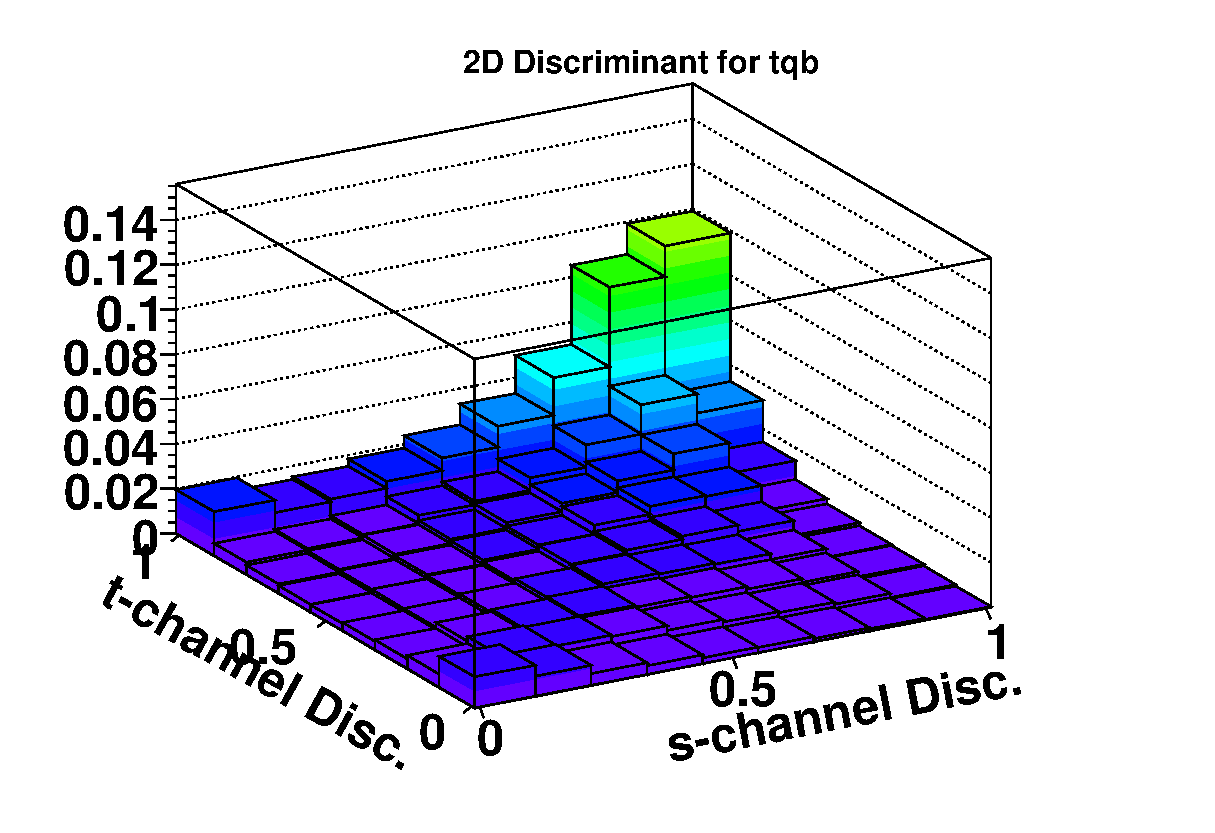
\includegraphics[width=0.32\textwidth]
{figures/performance/2D-Discriminant_tchannel}
\vspace{-0.1in}
\caption[tbtqwbbwcc]{2D-discriminant templates for: left, $tb$, and
right, $tqb$ Monte Carlo events.}
\label{tbtqb}
\end{figure}

\begin{figure}[!h!tbp]
\includegraphics[width=0.32\textwidth]
{figures/performance/2D-Discriminant_wbb}
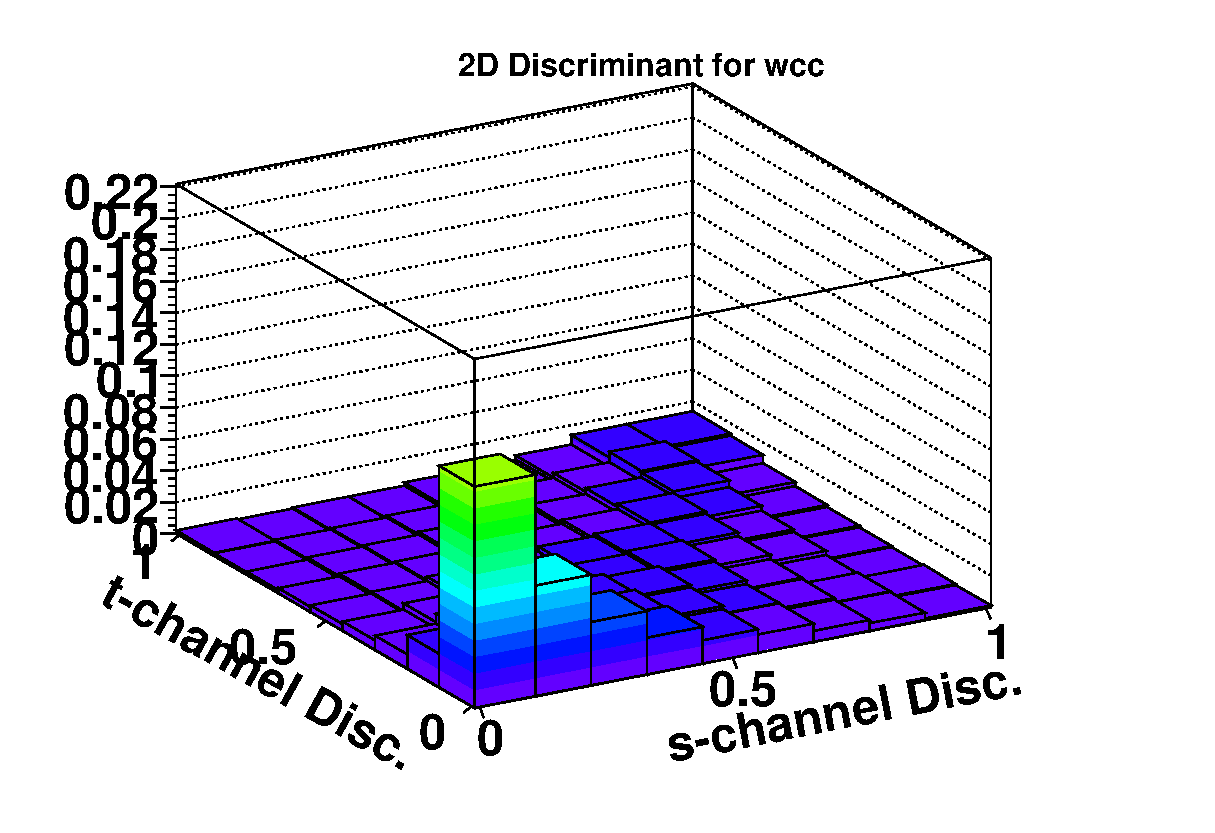
\includegraphics[width=0.32\textwidth]
{figures/performance/2D-Discriminant_wcc}
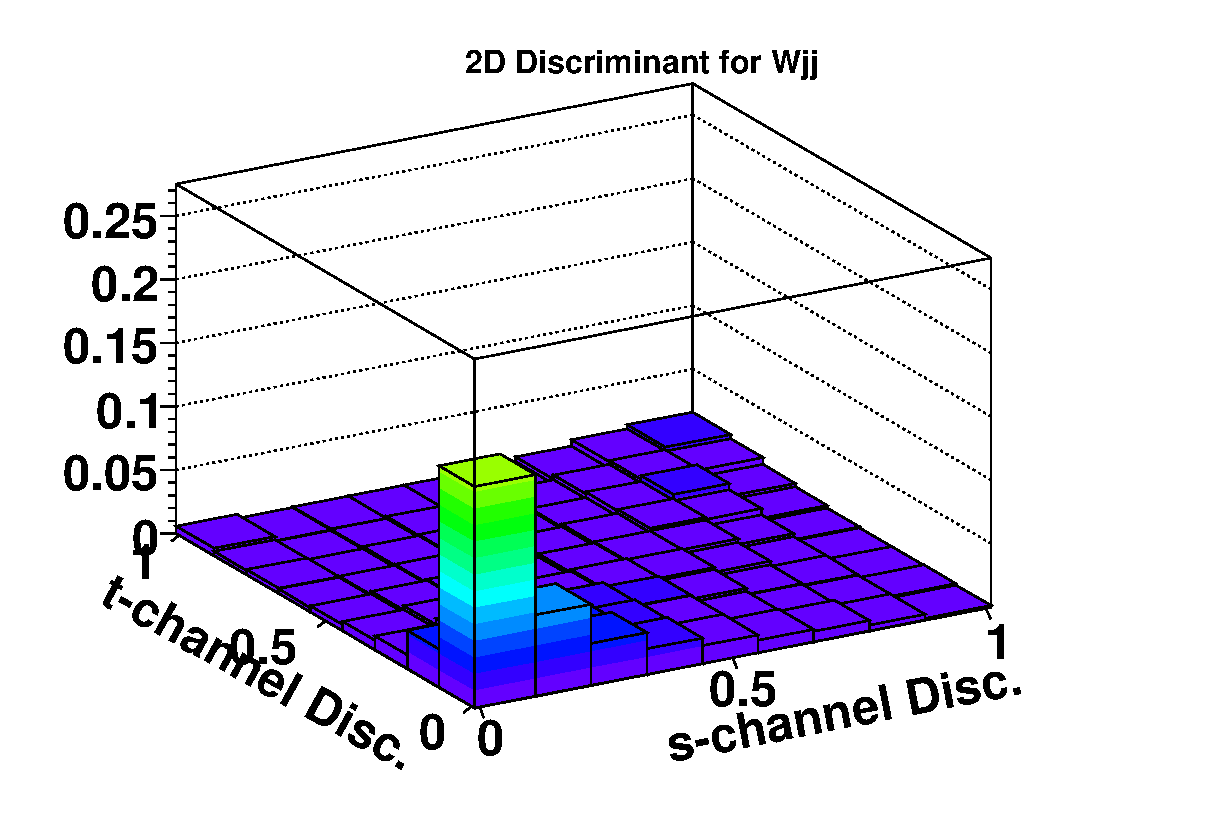
\includegraphics[width=0.32\textwidth]
{figures/performance/2D-Discriminant_wjj}
\vspace{-0.1in}
\caption[tbtqwbbwcc]{2D-discriminant templates for: left,
$Wbb$, middle, $Wcc$, and right, $Wjj$ Monte Carlo events.}
\label{wbbwccwjj}
\end{figure}

\begin{figure}[!h!tbp]
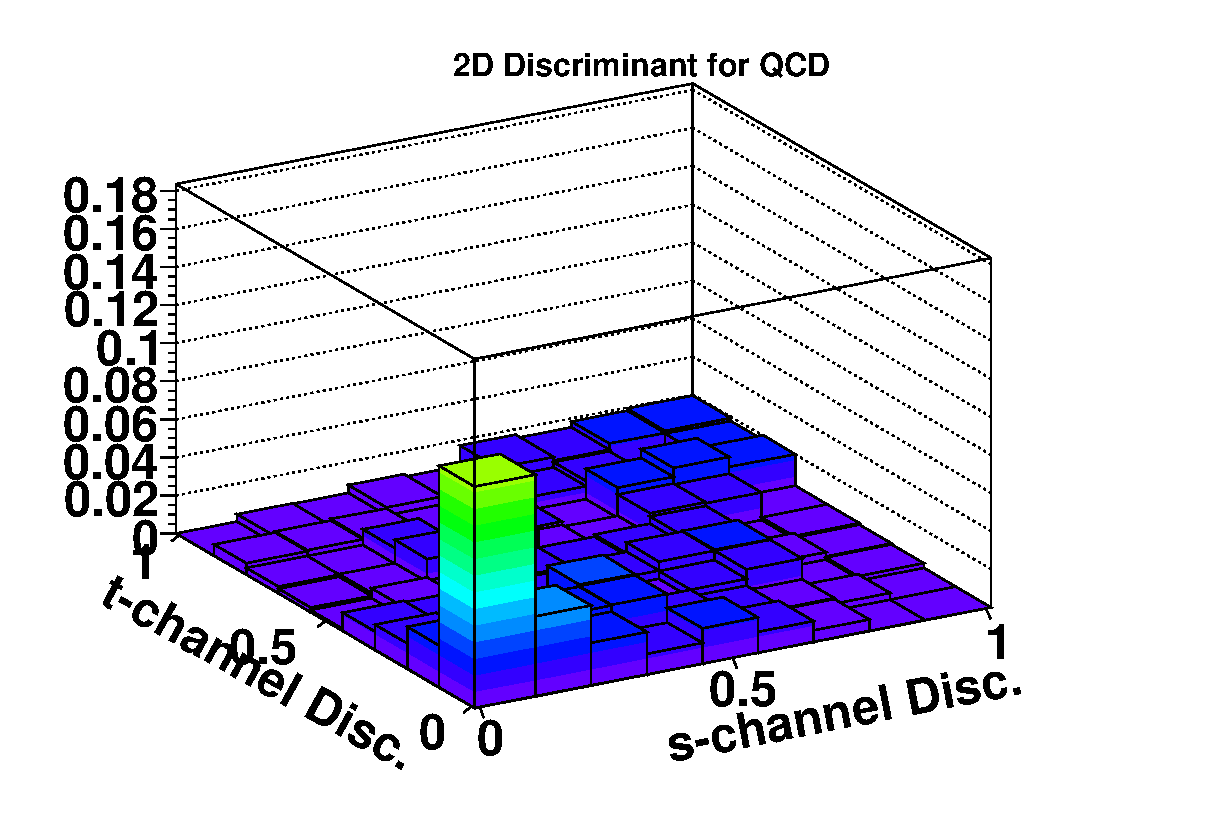
\includegraphics[width=0.32\textwidth]
{figures/performance/2D-Discriminant_qcd}
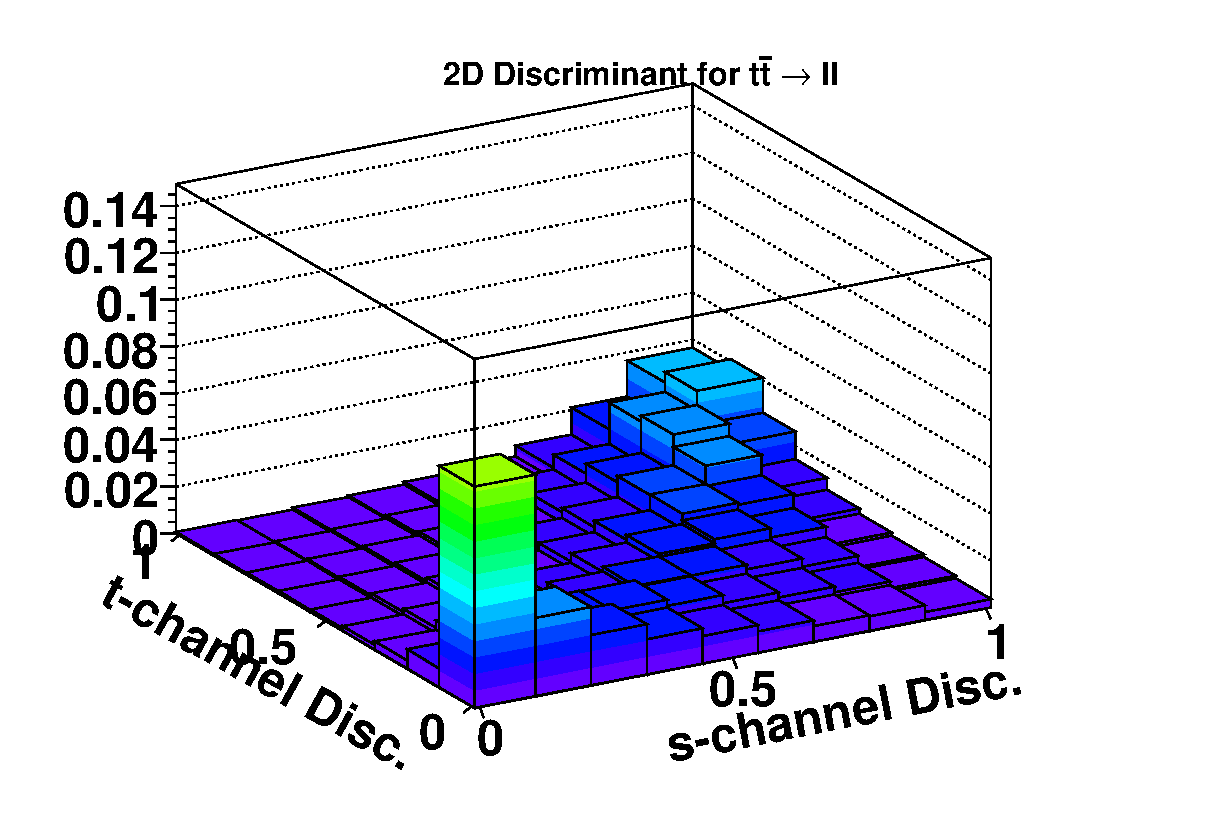
\includegraphics[width=0.32\textwidth]
{figures/performance/2D-Discriminant_dilepton}
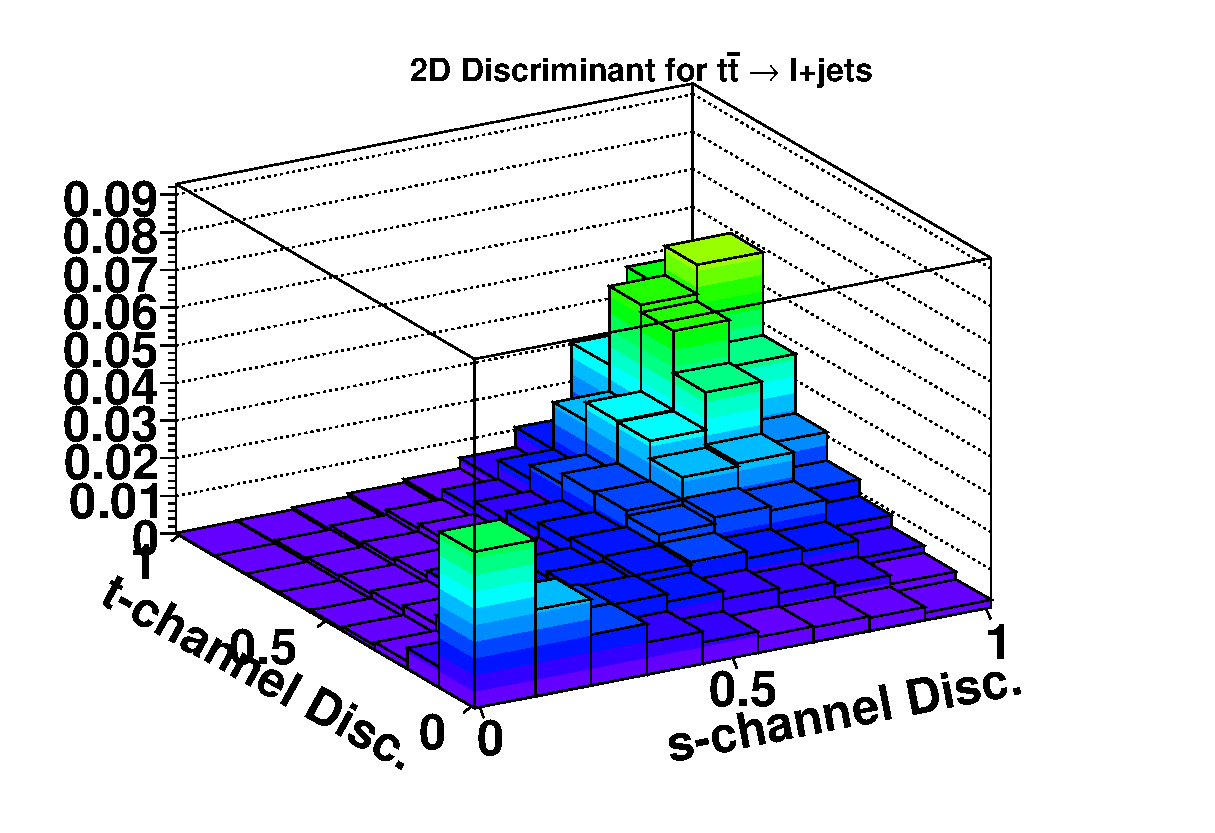
\includegraphics[width=0.32\textwidth]
{figures/performance/2D-Discriminant_lepjets}
\vspace{-0.1in}
\caption[wjjqcdtt]{2D-discriminant templates for: left,
multijets events, middle, $\dilepton$, and right, $\lepjets$ Monte
Carlo events.}
\label{qcdtt}
\end{figure}

